\newcommand{\flooderTagResultsAucTable}{
    \begin{table}[H]
        \centering
        \begin{tabular}{|p{2,8cm}||p{2,8cm} p{2,8cm} p{2,8cm}|}
            \hline
            Flooder Tag & ALOHA & Joint Embedding & Proposed Model \\
            \hline
            AUC-ROC & 0.985$\pm$0.001 & 0.985$\pm$0.000 & \textBF{0.987$\pm$0.000} \\
            \hline
        \end{tabular}
        \caption{AUC-ROC (Area Under Curve) of the different models for the \textbf{Flooder Tag} prediction task. Results were aggregated over \textBF{3} training runs with different weight initializations and minibatch orderings. Best results are shown in \textbf{bold}.} \label{tab:flooderTag_auc}
    \end{table}
}

\newcommand{\flooderTagResultsAtFprTable}{
    \begin{center}
        \begin{longtable}[c]{|p{3,2cm}||p{1,8cm} p{1,8cm} p{1,8cm} p{1,8cm} p{1,8cm}|}
            \hline
            Flooder Tag & \multicolumn{5}{c|}{{FPR}} \\
            & $10^{-5}$ & $10^{-4}$ & $10^{-3}$ & $10^{-2}$ & $10^{-1}$ \\
            \hline
            \endfirsthead

            \caption*{\raggedright ...continued from previous page} \\
            \hline
            Flooder Tag & \multicolumn{5}{c|}{\textbf{FPR}} \\
            & $10^{-5}$ & $10^{-4}$ & $10^{-3}$ & $10^{-2}$ & $10^{-1}$ \\
            \hline
            \endhead

            \caption*{\raggedleft ...continued on next page} \\
            \endfoot

            \caption{Mean and standard deviation results (TPR, Accuracy, Recall, Precision and F1-Score) of the different models for the \textbf{Flooder Tag} prediction task at different \textbf{FPR}s (\textit{False Positive Rates}). Results were aggregated over \textBF{3} training runs with different weight initializations and minibatch orderings. Best results are shown in \textbf{bold}. Under \textbf{TPR} results are also presented the percentage reduction in mean detection error and in ROC curve standard deviation introduced by the \textit{Proposed Model} with respect to both \textit{ALOHA} model and \textit{Joint Embedding}.} \label{tab:flooderTag_results_at_fpr} \\
            \endlastfoot

            \multicolumn{6}{|c|}{\textbf{TPR}} \\
            \hline
            ALOHA & 0.817$\pm$0.009 & \textBF{0.845$\pm$0.001} & \textBF{0.856$\pm$0.004} & 0.897$\pm$0.013 & 0.958$\pm$0.004 \\
            Joint Embedding & 0.828$\pm$0.011 & 0.833$\pm$0.005 & 0.833$\pm$0.005 & \textBF{0.914$\pm$0.001} & 0.957$\pm$0.001 \\
            Proposed Model & \textBF{0.829$\pm$0.005} & 0.833$\pm$0.009 & 0.833$\pm$0.009 & 0.912$\pm$0.002 & \textBF{0.962$\pm$0.003} \\
            \hline
            Error Reduction wrt \newline ALOHA & 6.6\% & -7.7\% & -16.0\% & 14.6\% & 9.5\% \\
            Error Reduction wrt \newline Joint Embedding & 0.6\% & 0.0\% & 0.0\% & -2.3\% & 11.6\% \\
            \hline
            Std Reduction wrt \newline ALOHA & 44.4\% & -800.0\% & -125.0\% & 84.6\% & 25.0\% \\
            Std Reduction wrt \newline Joint Embedding & 54.5\% & -80.0\% & -80.0\% & -100.0\% & -200.0\% \\
            \hline
            \multicolumn{6}{|c|}{\textbf{Accuracy}} \\
            \hline
            ALOHA & \textBF{1.000$\pm$0.000} & \textBF{1.000$\pm$0.000} & \textBF{0.999$\pm$0.000} & \textBF{0.990$\pm$0.000} & \textBF{0.900$\pm$0.000} \\
            Joint Embedding & \textBF{1.000$\pm$0.000} & \textBF{1.000$\pm$0.000} & \textBF{0.999$\pm$0.000} & \textBF{0.990$\pm$0.000} & \textBF{0.900$\pm$0.000} \\
            Proposed Model & \textBF{1.000$\pm$0.000} & \textBF{1.000$\pm$0.000} & \textBF{0.999$\pm$0.000} & \textBF{0.990$\pm$0.000} & \textBF{0.900$\pm$0.000} \\
            \hline
            \multicolumn{6}{|c|}{\textbf{Recall}} \\
            \hline
            ALOHA & 0.817$\pm$0.009 & \textBF{0.845$\pm$0.001} & \textBF{0.856$\pm$0.004} & 0.897$\pm$0.013 & 0.958$\pm$0.004 \\
            Joint Embedding & 0.828$\pm$0.011 & 0.833$\pm$0.005 & 0.833$\pm$0.005 & \textBF{0.914$\pm$0.001} & 0.957$\pm$0.001 \\
            Proposed Model & \textBF{0.829$\pm$0.005} & 0.833$\pm$0.009 & 0.833$\pm$0.009 & 0.912$\pm$0.002 & \textBF{0.962$\pm$0.003} \\
            \hline
            \multicolumn{6}{|c|}{\textbf{Precision}} \\
            \hline
            ALOHA & 0.994$\pm$0.000 & \textBF{0.938$\pm$0.001} & \textBF{0.609$\pm$0.001} & 0.140$\pm$0.002 & \textBF{0.017$\pm$0.000} \\
            Joint Embedding & \textBF{0.996$\pm$0.002} & \textBF{0.938$\pm$0.001} & 0.602$\pm$0.002 & \textBF{0.142$\pm$0.000} & \textBF{0.017$\pm$0.000} \\
            Proposed Model & \textBF{0.996$\pm$0.002} & 0.938$\pm$0.002 & 0.602$\pm$0.004 & \textBF{0.142$\pm$0.000} & \textBF{0.017$\pm$0.000} \\
            \hline
            \multicolumn{6}{|c|}{\textbf{F1 Score}} \\
            \hline
            ALOHA & 0.897$\pm$0.005 & \textBF{0.889$\pm$0.001} & \textBF{0.711$\pm$0.002} & 0.242$\pm$0.003 & \textBF{0.034$\pm$0.000} \\
            Joint Embedding & 0.904$\pm$0.006 & 0.882$\pm$0.002 & 0.699$\pm$0.003 & \textBF{0.246$\pm$0.000} & 0.033$\pm$0.000 \\
            Proposed Model & \textBF{0.905$\pm$0.003} & 0.882$\pm$0.006 & 0.699$\pm$0.006 & 0.245$\pm$0.000 & \textBF{0.034$\pm$0.000} \\
            \hline
        \end{longtable}
    \end{center}
}

\newcommand{\flooderTagResultsSummaryTable}{
    \begin{table}[H]
        \centering
        \begin{tabular}{|p{3,2cm}||p{1,8cm} p{1,8cm} p{1,8cm} p{1,8cm} p{1,8cm}|}
            \hline
            \multicolumn{6}{|c|}{Flooder Tag (at FPR $=1\%$)} \\
            \hline
            Model & TPR & Accuracy & Precision & Recall & F1 score \\
            \hline
            ALOHA & 0.897$\pm$0.013 & \textBF{0.990$\pm$0.000} & 0.140$\pm$0.002 & 0.897$\pm$0.013 & 0.242$\pm$0.003 \\
            Joint Embedding & \textBF{0.914$\pm$0.001} & \textBF{0.990$\pm$0.000} & \textBF{0.142$\pm$0.000} & \textBF{0.914$\pm$0.001} & \textBF{0.246$\pm$0.000} \\
            Proposed Model & 0.912$\pm$0.002 & \textBF{0.990$\pm$0.000} & \textBF{0.142$\pm$0.000} & 0.912$\pm$0.002 & 0.245$\pm$0.000 \\
            \hline
        \end{tabular}
        \caption{Summary of the mean and standard deviation results of the different models for the \textbf{Flooder Tag} prediction task at \textbf{FPR} $=1\%$. Results were aggregated over \textBF{3} training runs with different weight initializations and minibatch orderings. Best results are shown in \textbf{bold}.} \label{tab:flooderTag_result_summary}
    \end{table}
}

\newcommand{\flooderTagRocAloha}{
    \begin{figure}[H]
        \vspace*{-0.5cm}
        \centering
        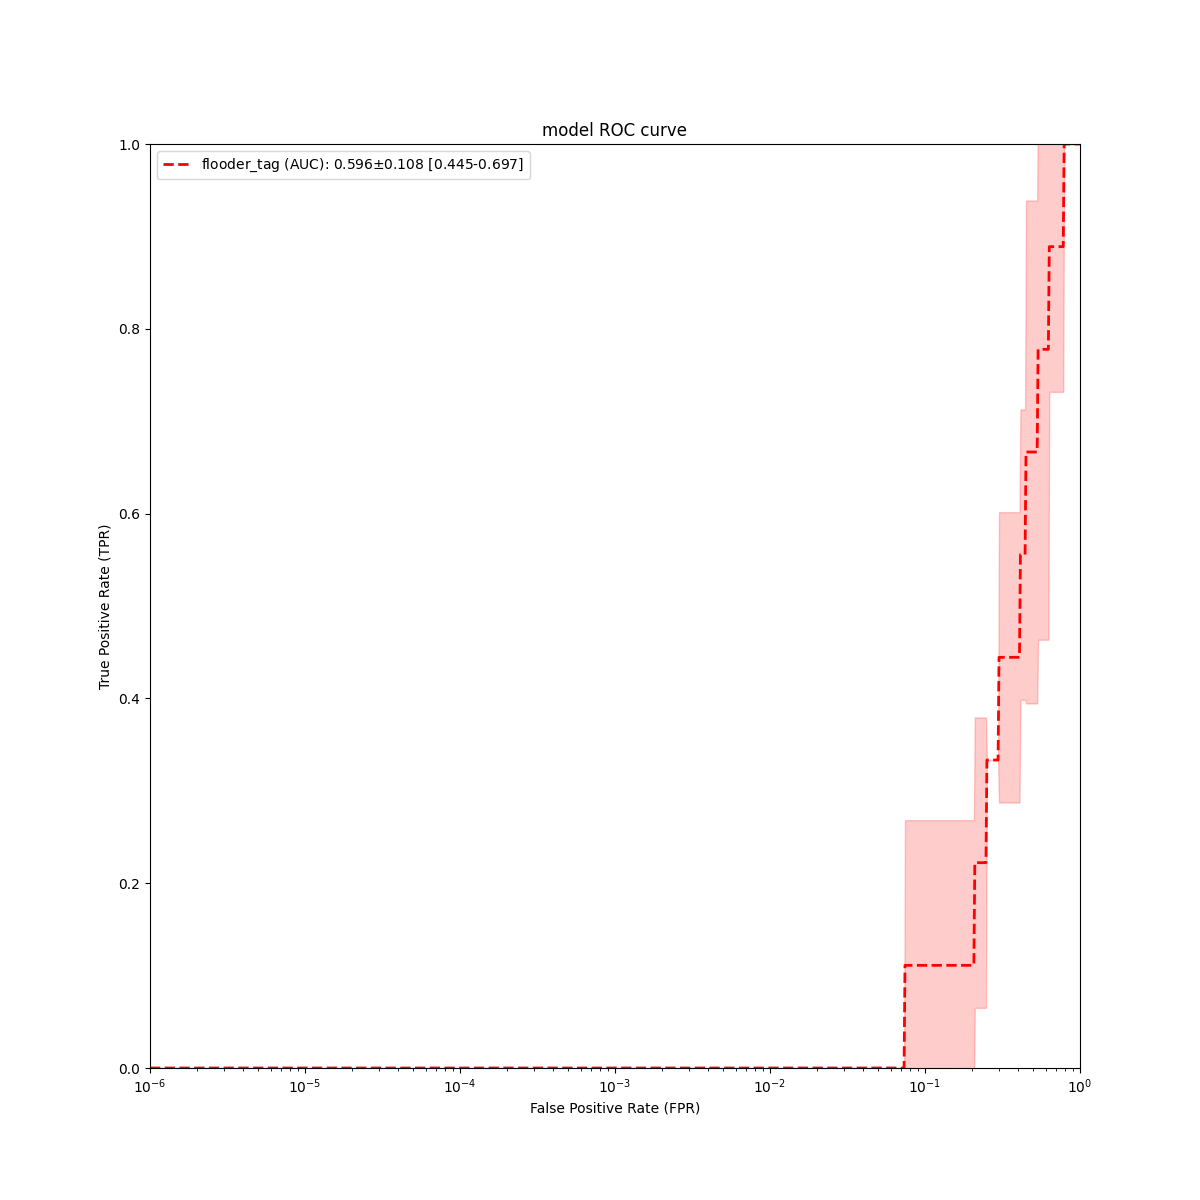
\includegraphics[width=0.6\textwidth]{./results/flooder_tag_roc_aloha.png}
        \vspace*{-0.2cm}
        \caption{ROC curve and AUC statistics of \textBF{ALOHA} model for the \textbf{Flooder Tag}. The line represents the \textit{mean} TPR at a given FPR, while the shaded region represents the \textit{standard deviation}. Statistics were computed over \textBF{3} training runs, each with random parameter initialization.}
        \label{fig:flooderTagRocAloha}
    \end{figure}
}

\newcommand{\flooderTagRocJointEmbedding}{
    \begin{figure}[H]
        \vspace*{-0.5cm}
        \centering
        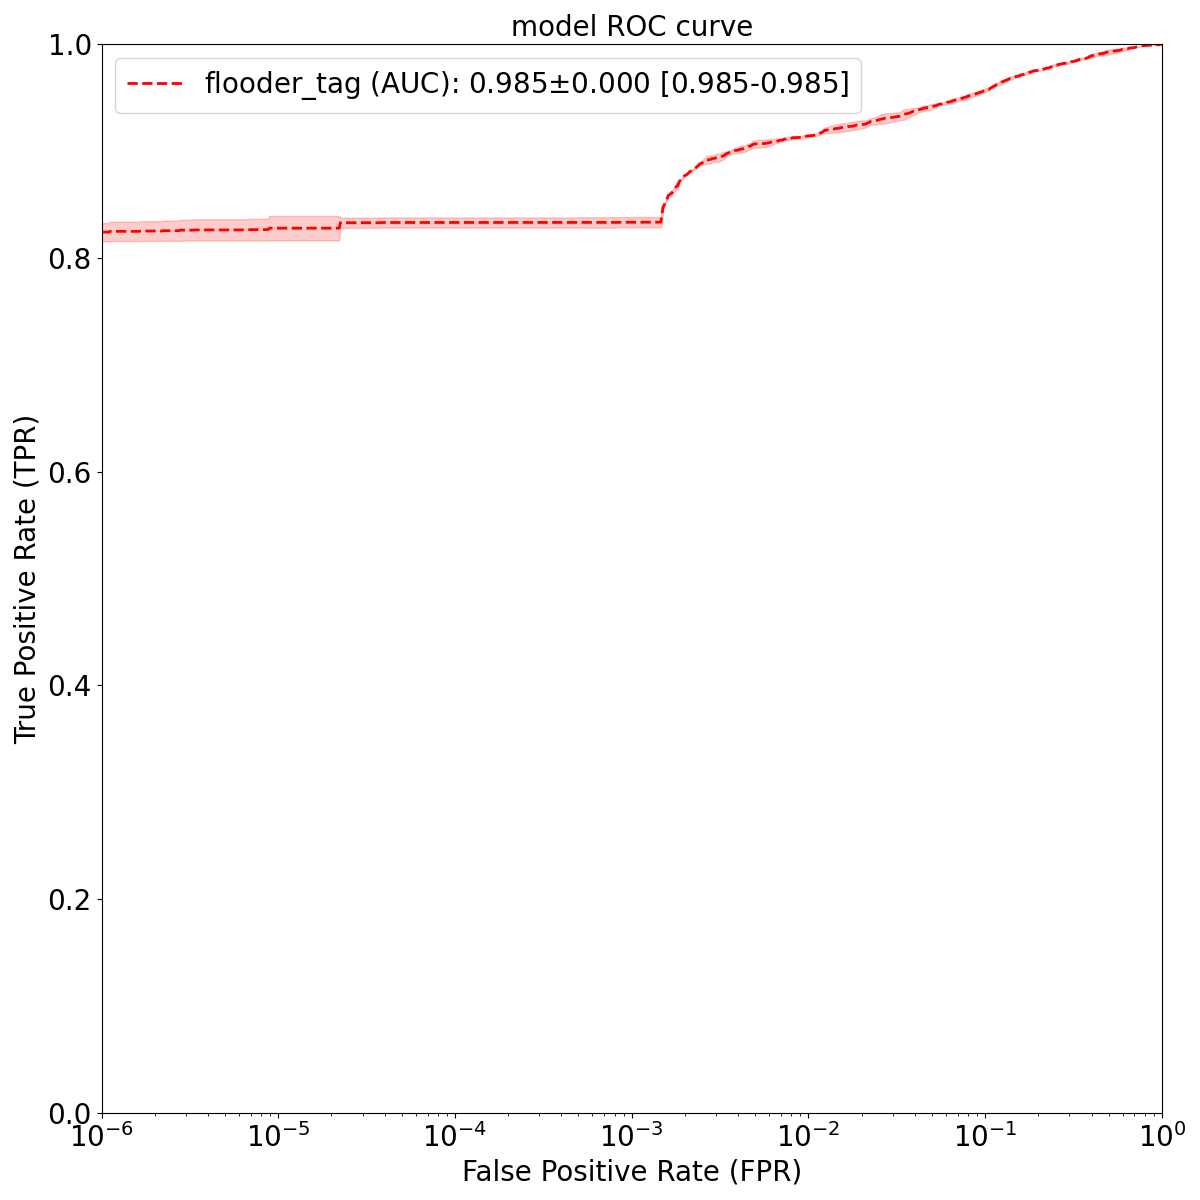
\includegraphics[width=0.6\textwidth]{./results/flooder_tag_roc_jointEmbedding.png}
        \vspace*{-0.2cm}
        \caption{ROC curve and AUC statistics of \textBF{Joint Embedding} model for the \textbf{Flooder Tag}. The line represents the \textit{mean} TPR at a given FPR, while the shaded region represents the \textit{standard deviation}. Statistics were computed over \textBF{3} training runs, each with random parameter initialization.}
        \label{fig:flooderTagRocJointEmbedding}
    \end{figure}
}

\newcommand{\flooderTagRocProposedMethod}{
    \begin{figure}[H]
        \vspace*{-0.5cm}
        \centering
        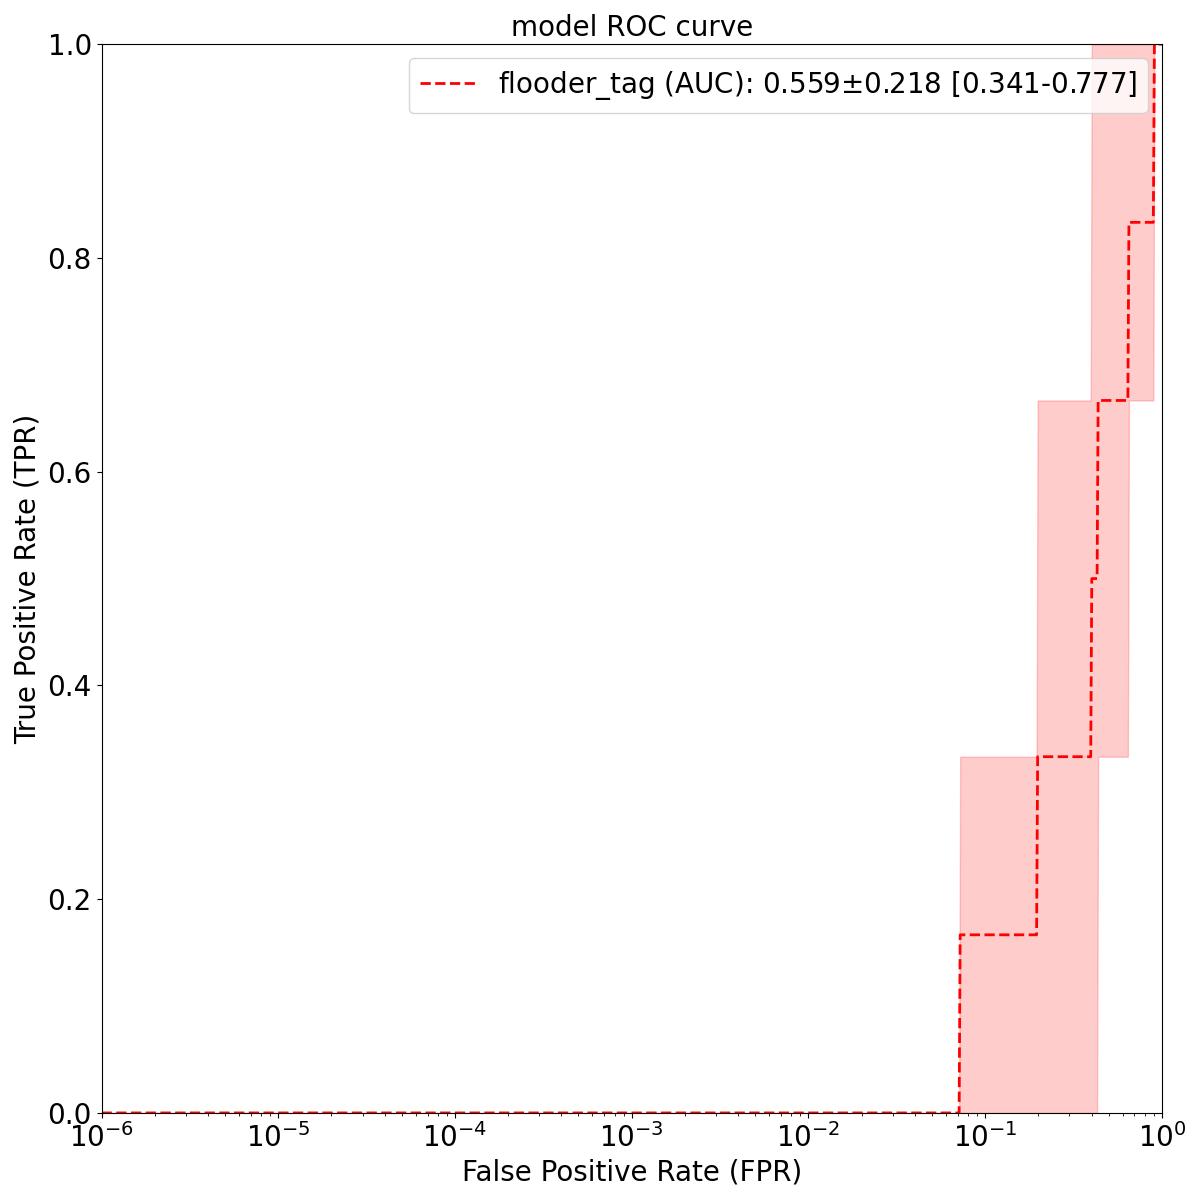
\includegraphics[width=0.6\textwidth]{./results/flooder_tag_roc_proposedModel.png}
        \vspace*{-0.2cm}
        \caption{ROC curve and AUC statistics of \textBF{Proposed Model} for the \textbf{Flooder Tag}. The line represents the \textit{mean} TPR at a given FPR, while the shaded region represents the \textit{standard deviation}. Statistics were computed over \textBF{3} training runs, each with random parameter initialization.}
        \label{fig:flooderTagRocProposedModel}
    \end{figure}
}
